%! Author = lazza
%! Date = 02/05/2022

\section{Branch prediction}\label{sec:branch-prediction}
When a branch is taken the \textbf{branch target address} (BTA) is stored in the PC instead of the address of the
next instruction in the sequential instruction stream.
The branch outcome and Branch Target Address are ready at the end of the EX stage, conditional branches are solved
when PC is updated at the end of the ME stage.
Control hazards reduce the performance from the ideal speedup gained by the pipelining since they can
make it necessary to stall the pipeline.

\begin{figure}[h]
    \centering
    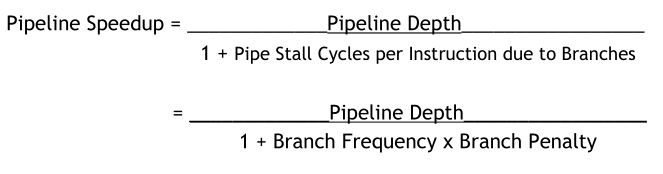
\includegraphics[scale = 0.35]{images/performace-impact-control-hazards}
    \caption{Performance impact by control hazards}
    \label{fig:performance-impact-by-control-hazards}
\end{figure}


\begin{figure}[h]
    \centering
    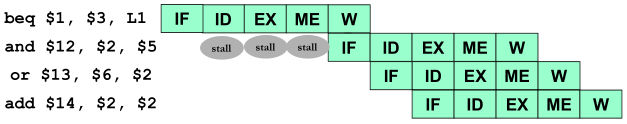
\includegraphics[scale = 0.4]{images/branch-without-forwarding}
    \caption{Branch stalls without forwarding}
    \label{fig:branch-stalls-without-forwarding}
\end{figure}

\begin{figure}[h]
    \centering
    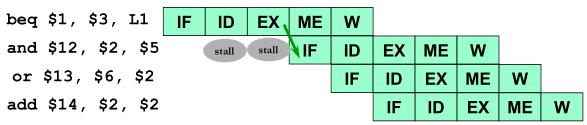
\includegraphics[scale = 0.4]{images/branch-with-forwarding}
    \caption{Branch stalls with forwarding}
    \label{fig:branch-stalls-with-forwarding}
\end{figure}

In order to reduce the speed penalty cause by the branch hazards we can use prediction techniques in order to guess
the next instruction to be executed.

\subsection{Static branch prediction}\label{subsec:static-branch-prediction}
Static branch prediction are at compile-time:
\begin{itemize}
    \item Branch always taken - No jump
    \item Branch always not taken\\ In theory always jump, but in reality we have to calculate the BTA before jumping
    and at this point there is no prediction to make (at least in the MIPS pipeline).
    \item Backward taken, forward not taken\\
    Based on the assumption that backward jumps (while and for loops) are taken and forward jumps (if statements) are
    not taken.
    \item Profile driven prediction\\
    We are going make several runs of our program and the choice is based on statistical data for each branch.
    \item Delayed Branch\\
    The compiler statically schedules and independent instruction in the branch delay slot, which is executed whether
    the branch is taken.
    %The independent instruction can belong also to the branch.
    There are three ways in which the branch delay slot can be scheduled:
        \subitem From before, the instruction in the delay slot is always executed.
        \subitem From target, this strategy is preferred when the branch is taken with high probability.
        \subitem From fall-through, this strategy is preferred when the branch is not taken with high probability. In
    this case the branch delay slot is scheduled from the not-taken fall-through path.
\end{itemize}

\begin{figure}[h]
    \centering
    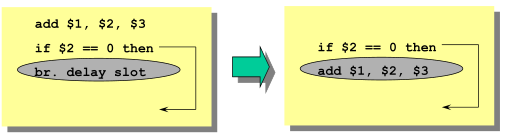
\includegraphics[scale = 0.4]{images/branch-delayed-from-before}
    \caption{Branch delayed - from before}
    \label{fig:branch-delayed-from-before}
\end{figure}

\begin{figure}[h]
    \centering
    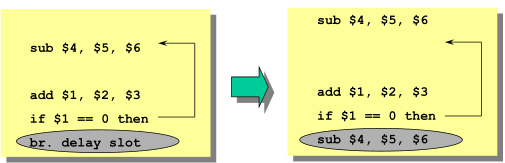
\includegraphics[scale = 0.4]{images/branch-delayed-from-target}
    \caption{Branch delayed - from target}
    \label{fig:branch-delayed-from-target}
\end{figure}

\begin{figure}[h]
    \centering
    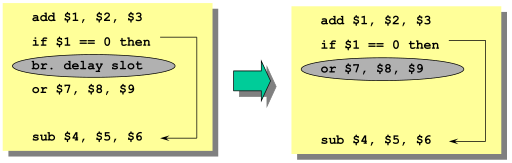
\includegraphics[scale = 0.4]{images/branch-delayed-from-fall-through}
    \caption{Branch delayed - from fall-through}
    \label{fig:branch-delayed-from-fall-through}
\end{figure}


\subsection{Dynamic branch prediction}\label{subsec:dynamic-branch-prediction}
Dynamic branch prediction happens at run-time by the hardware, and is based on two interacting mechaninsms:
\begin{itemize}
    \item Branch Outcome Predictor\\
    To predict the direction of a branch (i.e., taken or not taken).
    \subitem Branch History Table
    \item Branch Target Predictor\\
    To predict the branch target address in case of taken branch.
    \subitem Branch Target Buffer
\end{itemize}

\subsubsection{Branch Target Buffer}
The Branch Target Buffer (BTB or Branch Target Predictor) is a cache storing the predicted branch target address
for the next instruction after a branch.
We access the BTB in the IF stage using the instruction address of the fetched instruction (a possible branch) to
index the cache.

\begin{figure}[H]
    \centering
    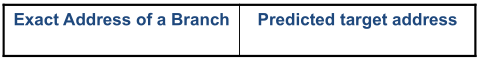
\includegraphics[scale = 0.4]{images/branch-target-buffer-entry}
    \caption{BTB entry}
    \label{fig:btb-entry}
\end{figure}

%In reality we cannot index all the possible branches since the BTB has a fixed size, the entry will not contain the
%exact address of a branch but only the last n-bits of the address, allowing the possibility for collisions.

\subsubsection{Branch History Table}
The Branch History Table (BHT or Branch Prediction Buffer) is indexed by the last k-bits of the branch address, meaning
that there are at most $2^k$ entries, with possible collisions, and each entry contains n-bits that says whether the
branch was recently taken.

\begin{figure}[H]
    \centering
    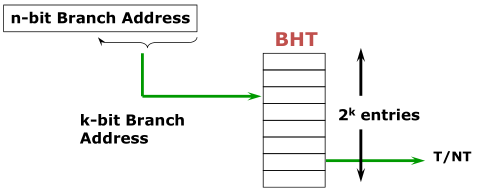
\includegraphics[scale = 0.4]{images/branch-history-table}
    \caption{Branch history table}
    \label{fig:branch-history-table}
\end{figure}

The 1-bit history table tells us if the last time the branch was taken or not taken (e.g., 0 and 1).
Differently from the profile drive prediction the BHT is updated whenever the branch is encountered.

For example:\\
0, prediction not taken, outcome not taken - no update\\
0, prediction not taken, outcome taken - update 0 to 1\\
0, prediction taken, outcome not taken - update 1 to 0\\

\begin{figure}[h]
    \centering
    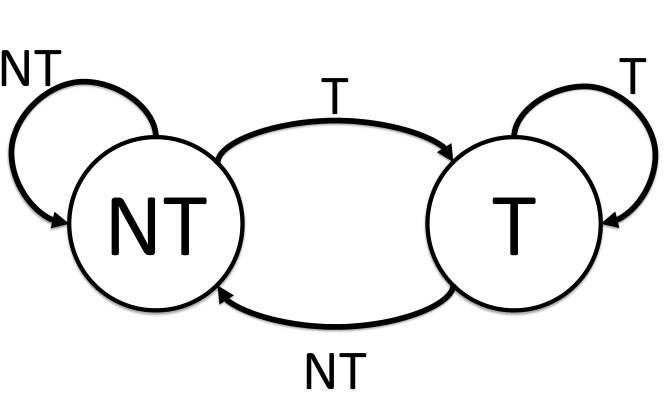
\includegraphics[scale = 0.15]{images/1-bit-BHT-automata}
    \caption{1-bit BHT automata}
    \label{fig:1-bit-BHT-automata}
\end{figure}

A misprediction occurs when:
\begin{itemize}
    \item[\textrightarrow] The prediction is incorrect for that branch
    \item[\textrightarrow] The same index has been referenced by two different branches, and the previous history
    refers to the other branch.
    To solve this problem it is enough to increase the number of rows in the BHT or to use a hashing function.
\end{itemize}

Among the n-bits BHT the \textbf{2-bit history table} is the best one because it is still small in size, it allows for speedy
updates maintaining
the prediction accuracy high, but differently from the 1-bit the prediction must miss twice before it is changed.
In a loop branch we do not need to change the prediction at the last iteration, thus increasing the speed in case of
nested loop such as the ones used to inspect matrices.

\begin{figure}[h]
    \centering
    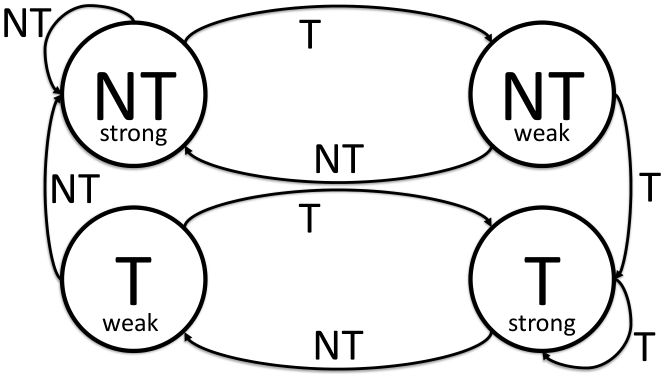
\includegraphics[scale = 0.2]{images/2-bit-BHT-automata}
    \caption{2-bit BHT automata}
    \label{fig:2-bit-BHT-automata}
\end{figure}

\begin{figure}[h]
    \centering
    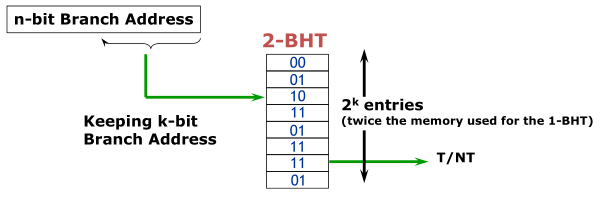
\includegraphics[scale = 0.3]{images/2-bit-BHT}
    \caption{2-bit BHT}
    \label{fig:2-bit-BHT}
\end{figure}


\subsubsection{Correlating Branch Predictor}
The idea behind is that the behaviour of recent branches are correlated, that is the recent behaviour of other
branches can influence the prediction of the current branch.
In general (m, n) correlating predictor records last m branches to choose from $2^m$ BHTs, each of which is a n-bit
predictor.
The branch prediction buffer can be indexed by
using a concatenation of low-order bits from the
branch address with m-bit global history (i.e.,
global history of the most recent m branches).

Example: a (2, 2) correlating predictor with 64 total entries;
6-bit index composed of: 2-bit global history and 4-bit low-
order branch address bits.

The (2,2) correlating branch predictor outperforms other predictors such as the 2-bit BHT\@.
\begin{figure}[H]
    \centering
    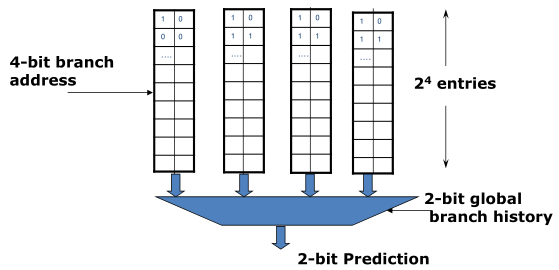
\includegraphics[scale = 0.4]{images/(2,2)-correlating-branch-predictor}
    \caption{(2,2) correlating branch predictor}
    \label{fig:(2,2)-correlating-branch-predictor}
\end{figure}

